% Rotaciones: girar es multiplicar
\chapter{Rotaciones: girar es multiplicar}\label{cap:rotaciones}

\section{La idea}

El capítulo~\ref{cap:antes-de-empezar} dejó el cuarto de vuelta como ejemplo de una matriz que
se lee como movimiento; ahora construimos todas las rotaciones a partir de tres afirmaciones:
un punto no es lo mismo que sus coordenadas, transformar es mover figuras y rotar es conservar
distancias alrededor de un centro.

\paragraph{Convenciones del capítulo.} El origen se llama \(o\) y los ángulos \(\theta\),
\emph{positivos en sentido antihorario}; el resto sigue la sección~\ref{sec:notacion}.

\begin{atencion}[Acimut no es \(\theta\)]
El acimut \(\mathrm{Az}\) se mide desde el norte y en sentido \emph{horario}; \(\theta\), desde el
este y en sentido \emph{antihorario}. Describen la misma dirección con números distintos:
\(\theta=90^\circ-\mathrm{Az}\) (módulo \(360^\circ\)), como deducimos en la sección~\ref{sec:acimut-campo}.
\end{atencion}

\subsection{El punto y sus coordenadas no son lo mismo}\label{sec:punto-coordenadas}

\unidadInteractiva{01a_punto_quieto}{Rotaciones I: el punto no se movió}{Explorá: girá los ejes con el deslizador \(\theta\) y mirá cómo cambian las coordenadas del mojón mientras el punto queda quieto.}

Un punto existe independientemente de cómo lo describamos; sus coordenadas aparecen recién
después de elegir un sistema de referencia.

\begin{definicion}[Sistema de coordenadas cartesiano]
Un sistema de coordenadas cartesiano del plano consiste en un punto \(o\), el \emph{origen};
dos rectas perpendiculares por \(o\), los \emph{ejes}, cada una con un sentido positivo; y una
\emph{unidad} de longitud. Si los vectores unitarios de los ejes son \(e_x,e_y\), las
coordenadas de un punto \(p\) son los únicos números \((x,y)\) tales que
\(p=o+x\,e_x+y\,e_y\). El sistema tiene \emph{orientación positiva} cuando \(e_y\) se obtiene
girando \(e_x\) un cuarto de vuelta en sentido antihorario.
\end{definicion}

Las coordenadas de un punto pueden cambiar, entonces, de dos maneras.

\begin{definicion}[Transformación activa y pasiva]
Una transformación es \emph{activa} cuando los ejes quedan fijos y el punto se mueve a otro
lugar. Es \emph{pasiva} cuando el punto queda fijo y lo que cambia es el sistema de
coordenadas con el que se lo describe.
\end{definicion}

\begin{center}
\begin{tikzpicture}[scale=.78]
  % panel izquierdo: ejes originales
  \draw[axisline,-{Latex[length=2mm]}] (-.4,0)--(4,0) node[right] {$x$};
  \draw[axisline,-{Latex[length=2mm]}] (0,-.4)--(0,2.6) node[above] {$y$};
  \draw[auxline] (3,0)--(3,1)--(0,1);
  \fill[teal] (3,1) circle (2.5pt) node[above right] {$p=(3,1)$};
  \fill[ink] (0,0) circle (1.6pt) node[below left] {$o$};
  % panel derecho: mismo punto, ejes girados 90 grados
  \begin{scope}[xshift=9.6cm]
    \draw[axisline,dotted] (-.4,0)--(4,0);
    \draw[axisline,dotted] (0,-.4)--(0,2.6);
    \draw[mainline,-{Latex[length=2mm]}] (0,-.4)--(0,2.6) node[above] {$x'$};
    \draw[mainline,-{Latex[length=2mm]}] (.4,0)--(-2.6,0) node[left] {$y'$};
    \draw[auxline] (3,1)--(0,1);
    \fill[teal] (3,1) circle (2.5pt) node[above right] {$p$: \((x',y')=(1,-3)\)};
    \fill[ink] (0,0) circle (1.6pt) node[below right] {$o$};
  \end{scope}
\end{tikzpicture}
\end{center}

\begin{ejemplo}[El mismo punto, dos descripciones]
Sea \(p=(3,1)\). Si giramos el \emph{punto} \(90^\circ\) alrededor de \(o\) (transformación
activa), su imagen tiene coordenadas \((-1,3)\) en los mismos ejes. Si en cambio giramos los
\emph{ejes} \(90^\circ\) y dejamos \(p\) quieto (transformación pasiva), los nuevos vectores
unitarios son \(e_{x'}=(0,1)\) y \(e_{y'}=(-1,0)\), y las nuevas coordenadas son
\(x'=p\cdot e_{x'}=1\), \(y'=p\cdot e_{y'}=-3\): el mismo punto se describe ahora como
\((1,-3)\). Las dos cuentas usan matrices inversas entre sí, \(R(90^\circ)\) y \(R(-90^\circ)\),
que se construyen en la sección~\ref{sec:rot-plano}.
\end{ejemplo}

\begin{idea}[La rotación sugiere las coordenadas polares]
Al girar alrededor de un centro, cada punto recorre una circunferencia. La familia de esas
circunferencias, junto con las semirrectas que salen del centro, forma las líneas coordenadas
de un sistema polar: la rotación misma sugiere una manera de poner coordenadas.
\end{idea}

\subsection{Qué significa transformar una figura}\label{sec:transformar}

\begin{definicion}[Transformación del plano]
Una \emph{transformación del plano} es una función \(F:\R^2\to\R^2\) que asigna a cada punto
\(p\) un punto imagen \(p'=F(p)\). Un \emph{punto fijo} de \(F\) es un punto \(q\) con
\(F(q)=q\).
\end{definicion}

Para comprender una transformación seguimos una figura sencilla, como un triángulo: adónde va
cada vértice, si se conservan longitudes, ángulos y paralelas, y si algún punto, recta o
dirección queda fijo.

\begin{center}
\begin{tikzpicture}[scale=.88]
  \coordinate (a) at (1,1);
  \coordinate (b) at (3.4,1.2);
  \coordinate (c) at (2,3.2);
  \coordinate (ap) at (7,1.4);
  \coordinate (bp) at (10.2,1.9);
  \coordinate (cp) at (8.2,4);
  \draw[teal,line width=1.1pt] (a)--(b)--(c)--cycle;
  \draw[rust,line width=1.1pt] (ap)--(bp)--(cp)--cycle;
  \foreach \p/\q in {a/ap,b/bp,c/cp}
    \draw[auxline,-{Latex[length=2mm]}] (\p)--(\q);
  \node[labelback,text=teal] at (2.1,.55) {figura original};
  \node[labelback,text=rust] at (8.7,1.0) {figura imagen};
\end{tikzpicture}
\end{center}

\begin{definicion}[Orientación]
Una transformación \emph{conserva la orientación} si todo triángulo cuyos vértices
\(a,b,c\) se recorren en sentido antihorario tiene una imagen \(a',b',c'\) que también se
recorre en sentido antihorario. Si el sentido se invierte, la transformación \emph{invierte}
la orientación (como un espejo).
\end{definicion}

Muchas transformaciones del apunte tienen la forma \(F(p)=Ap+t\): la matriz \(A\) transforma
direcciones y formas, y el vector \(t\) desplaza toda la figura sin deformarla
(sección~\ref{sec:transf-plano}).

\subsection{Rotar: conservar distancias alrededor de un centro}\label{sec:rotar}

\unidadInteractiva{01b_rotacion_plano}{Rotaciones II: la rotación en el plano}{Verificá: mové el deslizador \(\theta\) y comprobá que la distancia al centro no cambia.}

Una rotación mueve cada punto sobre una circunferencia cuyo centro es el centro de rotación,
y todos los puntos barren el mismo ángulo.

\begin{definicion}[Rotación del plano]
Sean \(c\) un punto y \(\theta\) un ángulo. La \emph{rotación de centro \(c\) y ángulo
\(\theta\)} es la transformación \(\rhoP{c,\theta}\) que deja fijo \(c\) y lleva cada punto
\(p\neq c\) al único punto \(p'\) tal que \(|p'-c|=|p-c|\) y el ángulo orientado que va de
\(p-c\) a \(p'-c\) es \(\theta\). Si \(c=o\) la llamamos \emph{rotación lineal} y la
escribimos \(R(\theta)\).
\end{definicion}

En dos dimensiones basta un centro y un ángulo. En tres dimensiones también se necesita un
\emph{eje}: una recta por el centro cuyos puntos quedan fijos; todo plano perpendicular al eje
gira como un plano bidimensional (sección~\ref{sec:rot-3d}).

\paragraph{Primera traducción algebraica.}
\[
  \rhoP{c,\theta}(p)=c+R(\theta)(p-c).
\]
El vector \(p-c\) expresa la posición vista desde el centro; \(R(\theta)\) lo gira, y sumar
\(c\) devuelve el resultado al sistema original.

\begin{idea}[El centro y un punto imagen determinan la rotación]
Una rotación deja fijo un punto, el centro, y conserva las distancias y los ángulos. Todo lo
demás se deduce de esa propiedad: fijado el centro y la imagen de un segundo punto, la imagen
de cualquier otro queda determinada.
\end{idea}

\section{Construcciones, cuentas y ejemplos}

\subsection{Transformaciones del plano}\label{sec:transf-plano}

\subsubsection{Transformaciones lineales y afines}

\begin{definicion}[Transformación lineal y afín]
Una transformación \(T:\R^2\to\R^2\) es \emph{lineal} si para todo par de vectores \(p,q\) y
todo número real \(s\)
\[
  T(p+q)=T(p)+T(q),\qquad T(s\,p)=s\,T(p).
\]
Una transformación \(F\) es \emph{afín} si existen una matriz \(A\) y un vector \(t\) tales
que \(F(p)=Ap+t\) para todo \(p\).
\end{definicion}

\begin{proposicion}\label{prop:lineal-origen}
Toda transformación lineal fija el origen. En consecuencia, una rotación con centro
\(c\neq o\) no es lineal.
\end{proposicion}

\begin{demostracion}
Con \(s=0\): \(T(o)=T(0\,p)=0\,T(p)=o\). Una rotación de centro \(c\neq o\) y ángulo
\(\theta\not\equiv0\) mueve el origen (lo lleva a otro punto de la circunferencia de centro
\(c\) que pasa por \(o\)), así que no puede ser lineal.
\end{demostracion}

Toda transformación lineal del plano es de la forma \(T(p)=Ap\): escribiendo
\(p=x\,e_x+y\,e_y\) y usando la linealidad, \(T(p)=x\,T(e_x)+y\,T(e_y)\), que es el producto
de la matriz cuyas columnas son \(T(e_x)\) y \(T(e_y)\) por la columna \((x,y)^T\). Esto
demuestra que \emph{las columnas de \(A\) son las imágenes de los vectores unitarios de los
ejes}.

\begin{ejemplo}[Columnas como imágenes de los ejes]
Sean
\[
A=\begin{pmatrix}2&0\\0&1\end{pmatrix},\qquad t=(1,0).
\]
La afinidad \(F(p)=Ap+t\) cumple \(Ae_x=(2,0)\) y \(Ae_y=(0,1)\): estira el eje \(x\) al doble y deja igual el eje
\(y\); después todo se corre una unidad hacia la derecha. El punto \((3,1)\) va a
\((2\cdot3+1,\,1)=(7,1)\). El origen va a \(t=(1,0)\), así que \(F\) no es lineal.
\end{ejemplo}

\subsection{Rotaciones en el plano}\label{sec:rot-plano}

{\small\vspace{1mm}\linkUnidad{01a_punto_quieto}{Simulación interactiva: Unidad 1 — Rotaciones I: el punto no se movió}\par}
{\small\vspace{1mm}\linkUnidad{01b_rotacion_plano}{Simulación interactiva: Unidad 2 — Rotaciones II: la rotación en el plano}\par}

\subsubsection{Matriz de rotación}

La rotación lineal de ángulo \(\theta\) lleva \(e_x=(1,0)\) a \((\cos\theta,\sin\theta)\) y
\(e_y=(0,1)\) a \((-\sin\theta,\cos\theta)\), que es \(e_x\) girado un cuarto de vuelta más.
Como las columnas de la matriz son las imágenes de los ejes, queda determinada.

\begin{definicion}[Matriz de rotación]
La \emph{matriz de rotación} de ángulo \(\theta\) es
\[
  R(\theta)=
  \begin{pmatrix}
    \cos\theta&-\sin\theta\\
    \sin\theta& \cos\theta
  \end{pmatrix}.
\]
Aplicada a \(p=(x,y)\):
\[
  R(\theta)p=
  \begin{pmatrix}
    x\cos\theta-y\sin\theta\\
    x\sin\theta+y\cos\theta
  \end{pmatrix}.
\]
\end{definicion}

\begin{center}
\begin{tikzpicture}[scale=1.0]
  \draw[axisline,-{Latex[length=2mm]}] (-.3,0)--(5.2,0) node[right] {$x$};
  \draw[axisline,-{Latex[length=2mm]}] (0,-.3)--(0,4.4) node[above] {$y$};
  \coordinate (p) at (4,1);
  \coordinate (q) at (2.2,3.5);
  \draw[auxline] (0,0)--(p);
  \draw[auxline] (0,0)--(q);
  \draw[mainline,-{Latex[length=2.6mm]}] (p)
    arc[start angle=14,end angle=58,radius=4.12];
  \fill[teal] (p) circle (2.5pt) node[below right] {$p$};
  \fill[rust] (q) circle (2.5pt) node[above right] {$R(\theta)p$};
  \node[text=teal] at (2.1,.75) {$\theta$};
\end{tikzpicture}
\end{center}

\begin{proposicion}[Propiedades de \(R(\theta)\)]\label{prop:propiedades-R}
Para todo par de ángulos \(\theta,\beta\):
\[
R(\theta)^TR(\theta)=I,\qquad
\det R(\theta)=1,\qquad
R(\beta)R(\theta)=R(\theta+\beta).
\]
En consecuencia \(R(\theta)\) conserva el producto interno, las longitudes, los ángulos y la
orientación.
\end{proposicion}

\begin{demostracion}
Las columnas de \(R(\theta)\) tienen norma \(\cos^2\theta+\sin^2\theta=1\) y su producto
interno es \(-\cos\theta\sin\theta+\sin\theta\cos\theta=0\); eso es \(R^TR=I\). El
determinante es \(\cos^2\theta+\sin^2\theta=1\). Para el producto, la primera columna de
\(R(\beta)R(\theta)\) es
\((\cos\beta\cos\theta-\sin\beta\sin\theta,\ \sin\beta\cos\theta+\cos\beta\sin\theta)
=(\cos(\theta+\beta),\sin(\theta+\beta))\) por las fórmulas de suma, y la segunda se obtiene
igual. Finalmente, \((Rp)\cdot(Rq)=p^TR^TRq=p\cdot q\), de modo que se conservan producto
interno, longitudes y ángulos; \(\det R>0\) significa que se conserva la orientación
(capítulo~\ref{cap:subespacios}).
\end{demostracion}

\begin{ejemplo}[Un cuarto de vuelta]
Para \(\theta=90^\circ=\pi/2\):
\[
R\left(\frac{\pi}{2}\right)=
\begin{pmatrix}0&-1\\1&0\end{pmatrix},
\qquad
R\left(\frac{\pi}{2}\right)\begin{pmatrix}3\\1\end{pmatrix}
=\begin{pmatrix}0\cdot3-1\cdot1\\1\cdot3+0\cdot1\end{pmatrix}
=\begin{pmatrix}-1\\3\end{pmatrix}.
\]
Es la transformación activa del ejemplo de la sección~\ref{sec:punto-coordenadas}; la pasiva
usa \(R(-\pi/2)=R(\pi/2)^T\) y da \((1,-3)\).
\end{ejemplo}

\subsubsection{Rotación alrededor de un centro cualquiera}

Para rotar alrededor de \(c\) trasladamos el centro al origen, rotamos y deshacemos la
traslación, y distribuyendo
\[
  \boxed{\rhoP{c,\theta}(p)=c+R(\theta)(p-c)=R(\theta)p+\bigl(I-R(\theta)\bigr)c}.
\]
Es una
transformación afín con parte lineal \(R(\theta)\) y traslación \(t=(I-R(\theta))c\), que es
distinta de cero si \(c\neq o\) y \(\theta\not\equiv0\).

\paragraph{Coordenadas homogéneas: primera presentación.}\label{sec:homogeneas-rotacion}
Para que la rotación alrededor de \(c\) sea, como la lineal, un solo producto por una matriz,
agregamos una tercera coordenada igual a \(1\): el punto \((x,y)\) se escribe \((x,y,1)^T\).
La rotación lineal pasa a ser la matriz \(3\times3\)
\[
\begin{pmatrix}
\cos\theta&-\sin\theta&0\\
\sin\theta&\cos\theta&0\\
0&0&1
\end{pmatrix},
\]
que hace con \((x,y)\) lo mismo que \(R(\theta)\) y deja el \(1\) en su lugar, y la rotación
alrededor de \(c\) se escribe con una sola matriz:
\[
H_{c,\theta}=
\begin{pmatrix}
R(\theta) & (I-R(\theta))c\\
0\ \ 0 & 1
\end{pmatrix}.
\]
La última columna guarda la traslación \((I-R(\theta))c\) y la última fila, \((0\ 0\ 1)\),
conserva el \(1\). Componer rotaciones es multiplicar estas matrices. Son las coordenadas
homogéneas, cuya teoría completa está en la sección~\ref{sec:homogeneas}.

\begin{center}
\begin{tikzpicture}[scale=.95]
  \coordinate (c) at (3,2.2);
  \coordinate (p) at (6.2,1.5);
  \coordinate (q) at (5.4,4.3);
  \draw[auxline] (c)--(p);
  \draw[auxline] (c)--(q);
  \draw[mainline,-{Latex[length=2.6mm]}] (p)
    arc[start angle=-12,end angle=42,radius=3.28];
  \fill[ink] (c) circle (2.7pt) node[below left] {$c$};
  \fill[teal] (p) circle (2.5pt) node[below right] {$p$};
  \fill[rust] (q) circle (2.5pt) node[above right] {$\rhoP{c,\theta}(p)$};
  \draw[muted,dotted] (0,0)--(7.6,0);
  \draw[muted,dotted] (0,0)--(0,5);
  \fill[muted] (0,0) circle (1.8pt) node[below left] {$o$};
\end{tikzpicture}
\end{center}

\begin{ejemplo}[Rotar \(p=(3,1)\) un ángulo de \(30^\circ\) alrededor de \(c=(1,1)\)]\label{ej:rot30}
\emph{Paso 1, ver el punto desde el centro.} \(p-c=(3-1,\,1-1)=(2,0)\).

\emph{Paso 2, girar.} Con \(\cos30^\circ=\sqrt3/2\approx0{,}866\) y \(\sin30^\circ=1/2\):
\[
R(30^\circ)(p-c)=
\begin{pmatrix}\sqrt3/2&-1/2\\[2pt]1/2&\sqrt3/2\end{pmatrix}
\begin{pmatrix}2\\0\end{pmatrix}
=\begin{pmatrix}\sqrt3\\1\end{pmatrix}
\approx\begin{pmatrix}1{,}732\\1\end{pmatrix}.
\]

\emph{Paso 3, volver al sistema original.}
\(p'=c+(\sqrt3,1)=(1+\sqrt3,\,2)\approx(2{,}732;\ 2)\).

\emph{Verificación.} \(|p-c|=|(2,0)|=2\) y \(|p'-c|=|(\sqrt3,1)|=\sqrt{3+1}=2\): el punto
quedó sobre la circunferencia de radio \(2\) y centro \(c\). Con la forma afín se llega a lo
mismo: \((I-R(30^\circ))c\approx(0{,}634;\,-0{,}366)\) y
\(R(30^\circ)p+(0{,}634;\,-0{,}366)\approx(2{,}732;\ 2)\).

\begin{center}
\begin{tikzpicture}[scale=1.25]
  \draw[axisline,-{Latex[length=2mm]}] (-.3,0)--(4.4,0) node[right] {$x$};
  \draw[axisline,-{Latex[length=2mm]}] (0,-.3)--(0,3.4) node[above] {$y$};
  \coordinate (c) at (1,1);
  \coordinate (p) at (3,1);
  \coordinate (pp) at (2.732,2);
  \draw[auxline] (c) circle (2);
  \draw[auxline] (c)--(p);
  \draw[auxline] (c)--(pp);
  \draw[mainline,-{Latex[length=2.4mm]}] (p) arc[start angle=0,end angle=30,radius=2];
  \draw[gold,line width=.9pt] ($(c)+(.7,0)$) arc[start angle=0,end angle=30,radius=.7];
  \node[text=gold!80!ink] at ($(c)+(15:1.0)$) {$30^\circ$};
  \fill[ink] (c) circle (2.4pt) node[below left] {$c=(1,1)$};
  \fill[teal] (p) circle (2.4pt) node[below right] {$p=(3,1)$};
  \fill[rust] (pp) circle (2.4pt) node[above right] {$p'\approx(2{,}732;\,2)$};
  \node[labelback,text=muted,font=\small] at (1,-1.25) {radio \(2\)};
\end{tikzpicture}
\end{center}
\end{ejemplo}

\subsection{Orientar una estación total: acimut y ángulo matemático}\label{sec:acimut-campo}

Una estación total mide direcciones horizontales sobre un limbo graduado. Al estacionar el
instrumento, el cero del limbo apunta a una dirección arbitraria, de modo que cada lectura
\(\mathrm{Lec}\) es la dirección medida desde ese cero, en sentido horario. Para pasar a
acimutes se visa un punto de referencia cuyo acimut \(\mathrm{Az}_{\text{ref}}\) se conoce y se calcula la \emph{corrección de
orientación} \(\kappa\)
\[
\kappa=\mathrm{Az}_{\text{ref}}-\mathrm{Lec}_{\text{ref}}\pmod{360^\circ},
\qquad
\mathrm{Az}_i=\mathrm{Lec}_i+\kappa\pmod{360^\circ}.
\]
Sumar la misma constante a todas las lecturas es girar el haz de direcciones completo: una
rotación horaria de ángulo \(\kappa\), que con \(\theta\) antihorario es \(R(-\kappa)\).

\begin{proposicion}[Acimut y ángulo matemático]\label{prop:acimut-theta}
Si el eje \(x\) apunta al este y el eje \(y\) al norte, la dirección de acimut \(\mathrm{Az}\)
tiene ángulo matemático
\[
\theta=90^\circ-\mathrm{Az}\pmod{360^\circ},
\]
y un tramo de longitud \(d\) en esa dirección tiene componentes
\((\Delta E,\Delta N)=d\,(\sin\mathrm{Az},\cos\mathrm{Az})=d\,(\cos\theta,\sin\theta)\).
\end{proposicion}

\begin{demostracion}
El norte tiene \(\theta=90^\circ\) y \(\mathrm{Az}=0^\circ\). Aumentar el acimut en cierto ángulo
es girar en sentido horario, es decir, disminuir \(\theta\) en ese mismo ángulo; por lo tanto
\(\theta=90^\circ-\mathrm{Az}\). Las componentes salen de
\(\cos(90^\circ-\mathrm{Az})=\sin\mathrm{Az}\) y \(\sin(90^\circ-\mathrm{Az})=\cos\mathrm{Az}\).
\end{demostracion}

\begin{ejemplo}[Orientar una lectura]
Desde una estación se visa la referencia con lectura \(\mathrm{Lec}_{\text{ref}}=352{,}5^\circ\)
y acimut conocido \(\mathrm{Az}_{\text{ref}}=40^\circ\). La corrección es
\(\kappa=40^\circ-352{,}5^\circ\equiv47{,}5^\circ\). Un punto \(q\) leído en
\(\mathrm{Lec}_q=100^\circ\) tiene \(\mathrm{Az}_q=147{,}5^\circ\) y, por la
proposición~\ref{prop:acimut-theta}, \(\theta_q=90^\circ-147{,}5^\circ=-57{,}5^\circ\equiv302{,}5^\circ\).
Con una distancia horizontal \(d=50\) m:
\(\Delta E=50\sin147{,}5^\circ\approx26{,}865\) m y \(\Delta N=50\cos147{,}5^\circ\approx-42{,}170\) m;
con \(\theta\) se obtienen los mismos valores, \(50\cos(-57{,}5^\circ)\) y \(50\sin(-57{,}5^\circ)\).

\begin{center}
\begin{tikzpicture}[scale=1.1]
  \draw[axisline,-{Latex[length=2mm]}] (-2.2,0)--(2.6,0) node[right] {$E$ (eje \(x\))};
  \draw[axisline,-{Latex[length=2mm]}] (0,-2.2)--(0,2.4) node[above] {$N$ (eje \(y\))};
  \draw[mainline,-{Latex[length=2.4mm]}] (0,0)--(-57.5:2.2) node[below right] {$q$};
  \draw[rust,line width=.9pt,-{Latex[length=2mm]}] (90:1.3) arc[start angle=90,end angle=-57.5,radius=1.3];
  \node[labelback,text=rust] at (40:1.75) {\(\mathrm{Az}=147{,}5^\circ\) (horario)};
  \draw[gold,line width=.9pt,-{Latex[length=2mm]}] (0:.65) arc[start angle=0,end angle=-57.5,radius=.65];
  \node[labelback,text=gold!80!ink,font=\small] at (-1.55,-1.0) {\(\theta=-57{,}5^\circ\equiv302{,}5^\circ\)};
  \fill[ink] (0,0) circle (1.8pt);
\end{tikzpicture}
\end{center}
\end{ejemplo}

\subsection{Rotaciones y números complejos}\label{sec:rot-complejos}

Identificando \((x,y)\in\R^2\) con \(z=x+iy\in\mathbb C\), la fórmula de Euler
\[
  e^{i\theta}=\cos\theta+i\sin\theta
\]
(que se obtiene comparando las series de Taylor de las tres funciones) permite escribir la
rotación lineal como
\[
  z'=e^{i\theta}z.
\]
Si se multiplica por un complejo general \(k\,e^{i\theta}\) con \(k>0\), el módulo \(k\)
produce una homotecia de razón \(k\) y el argumento \(\theta\) produce una rotación:
\[
  z'=k\,e^{i\theta}z.
\]

\begin{ejemplo}[El cuarto de vuelta en forma compleja]
Para \(z=3+i\) y \(\theta=\pi/2\), \(e^{i\pi/2}=i\) y \(z'=i(3+i)=3i+i^2=-1+3i\), que
corresponde al punto \((-1,3)\): el mismo resultado que \(R(\pi/2)(3,1)\).
\end{ejemplo}

\begin{idea}[Relación entre la forma compleja y la matricial]
Multiplicar por \(a+ib\) es aplicar la matriz
\(\left(\begin{smallmatrix}a&-b\\b&a\end{smallmatrix}\right)\) (ladrillo 2 de la
subsección~\ref{sec:desaprender}): una familia de transformaciones lineales reales con dos
parámetros en lugar de cuatro, cerrada por producto.
\end{idea}

\subsection{Rotaciones en tres dimensiones}\label{sec:rot-3d}

\unidadInteractiva{01c_rotaciones_3d}{Rotaciones III: tres ejes y el orden importa}{Explorá: fijá \(\alpha,\beta,\gamma\), cambiá el orden de los ejes en el menú y comprobá que el resultado cambia.}

\subsubsection{Rotaciones elementales}

Una rotación alrededor de un eje coordenado deja fija la coordenada de ese eje y gira el
plano perpendicular como una rotación plana, con sentido positivo dado por la regla de la mano
derecha (el pulgar apunta en el sentido positivo del eje).

\begin{definicion}[Rotaciones elementales]
Las rotaciones de ángulo \(\theta\) alrededor de los ejes \(x\), \(y\), \(z\) son
\[
R_x(\theta)=
\begin{pmatrix}
1&0&0\\0&\cos\theta&-\sin\theta\\0&\sin\theta&\cos\theta
\end{pmatrix},\quad
R_y(\theta)=
\begin{pmatrix}
\cos\theta&0&\sin\theta\\0&1&0\\-\sin\theta&0&\cos\theta
\end{pmatrix},\quad
R_z(\theta)=
\begin{pmatrix}
\cos\theta&-\sin\theta&0\\
\sin\theta& \cos\theta&0\\
0&0&1
\end{pmatrix}.
\]
\end{definicion}

El signo cambiado de \(R_y\) se debe a que el plano perpendicular a \(y\), recorrido según la
mano derecha, es el plano \(zx\) (de \(z\) hacia \(x\)) y no el \(xz\). La construcción
geométrica completa de las tres matrices, con figuras, está en el
apéndice~\ref{ap:rot3d}.

\subsubsection{El orden importa}\label{sec:orden-importa}

En el plano, \(R(\beta)R(\theta)=R(\theta+\beta)=R(\theta)R(\beta)\): las rotaciones lineales
conmutan. En el espacio no.

\begin{ejemplo}[Dos cuartos de vuelta en distinto orden]
Tomemos \(e_z=(0,0,1)^T\) y giros de \(90^\circ\). La tercera columna de
\(R_x(\pi/2)\) es \((0,-\sin\tfrac{\pi}{2},\cos\tfrac{\pi}{2})^T=(0,-1,0)^T\), así que
\(R_x(\pi/2)e_z=-e_y\); además \(R_y\) deja fijo \(e_y\). Entonces
\[
R_y\left(\frac{\pi}{2}\right)
R_x\left(\frac{\pi}{2}\right)e_z
=R_y\left(\frac{\pi}{2}\right)(-e_y)
=-e_y.
\]
Al invertir el orden, la tercera columna de \(R_y(\pi/2)\) es \((1,0,0)^T\) y \(R_x\) deja
fijo \(e_x\):
\[
R_x\left(\frac{\pi}{2}\right)
R_y\left(\frac{\pi}{2}\right)e_z
=R_x\left(\frac{\pi}{2}\right)e_x
=e_x.
\]
Como \(-e_y\neq e_x\), \(R_yR_x\neq R_xR_y\). La diferencia no es un error numérico: es una
propiedad geométrica de las rotaciones espaciales.
\end{ejemplo}

\subsection{Aplicación topográfica: acimut y estación total}\label{sec:rotaciones-aplicacion}

Seguimos ahora la cuenta completa de un \emph{radiado}: desde una estación de coordenadas
conocidas se miden, para cada punto nuevo, una distancia horizontal \(d\) y un ángulo
horizontal \(\beta\), contado en sentido horario desde la visual a un punto de referencia; con
eso se calculan las coordenadas del punto. Cada paso es una rotación, y por eso las distancias
no se alteran.

\paragraph{Los datos.} La estación es el punto \(A\) y la referencia es el punto \(B\), ambos
con coordenadas Gauss-Krüger de la faja~5, en metros:
\[
A=(E_A,N_A)=(5\,412\,837{,}425;\ 6\,171\,254{,}318),\qquad
B=(5\,413\,096{,}512;\ 6\,171\,618{,}903).
\]
Con el cero de la medición en la visual a \(B\), se observan dos puntos \(P\) y \(Q\):
\[
\beta_P=47^\circ\,23'\,15'',\quad d_P=86{,}452\text{ m};\qquad
\beta_Q=128^\circ\,41'\,38'',\quad d_Q=143{,}217\text{ m}.
\]
Los ángulos sexagesimales se pasan a grados decimales dividiendo los minutos por \(60\) y los
segundos por \(3600\), y a radianes multiplicando por \(\pi/180\):
\[
\beta_P=47+\tfrac{23}{60}+\tfrac{15}{3600}=47{,}387500^\circ=0{,}827068\text{ rad},\qquad
\beta_Q=128+\tfrac{41}{60}+\tfrac{38}{3600}=128{,}693889^\circ=2{,}246132\text{ rad}.
\]

\paragraph{El acimut de referencia sale de las coordenadas.} El acimut de \(A\) hacia \(B\) es
el ángulo, medido desde el norte en sentido horario, de la dirección
\((\Delta E,\Delta N)=B-A=(259{,}087;\ 364{,}585)\) m. Por la
proposición~\ref{prop:acimut-theta}, \(\Delta E=d\sin\mathrm{Az}\) y
\(\Delta N=d\cos\mathrm{Az}\), de modo que \(\tan\mathrm{Az}=\Delta E/\Delta N\). Pero la
tangente tiene período \(180^\circ\): el cociente no distingue una dirección de su opuesta. Hay
que mirar los signos de \(\Delta E\) y \(\Delta N\) por separado, que es lo que hace la función
de dos argumentos
\[
\mathrm{Az}_{AB}=\operatorname{atan2}(\Delta E,\Delta N)\pmod{360^\circ},
\]
con el \emph{este en el primer lugar}: es el orden inverso al de la convención matemática
\(\operatorname{atan2}(y,x)\), justamente porque el acimut parte del norte. Aquí ambos
incrementos son positivos (primer cuadrante) y
\[
\mathrm{Az}_{AB}=35{,}398948^\circ=35^\circ\,23'\,56{,}2'',\qquad
\overline{AB}=447{,}268\text{ m}.
\]
El \emph{acimut inverso}, de \(B\) hacia \(A\), corresponde al vector opuesto
\(A-B=-(B-A)\); invertir un vector es girarlo media vuelta, así que
\[
\mathrm{Az}_{BA}=\mathrm{Az}_{AB}\pm180^\circ=215{,}398948^\circ=215^\circ\,23'\,56{,}2'',
\]
eligiendo el signo que deja el resultado entre \(0^\circ\) y \(360^\circ\).

\paragraph{Orientar es componer rotaciones.} Como \(\beta\) se cuenta desde la visual a \(B\)
en el mismo sentido que el acimut,
\[
\mathrm{Az}_P=\mathrm{Az}_{AB}+\beta_P=82{,}786448^\circ=82^\circ\,47'\,11{,}2'',\qquad
\mathrm{Az}_Q=\mathrm{Az}_{AB}+\beta_Q=164{,}092837^\circ=164^\circ\,05'\,34{,}2'',
\]
siempre módulo \(360^\circ\) (si la suma pasa de \(360^\circ\), se resta una vuelta).

\begin{proposicion}[El radiado es una rotación]\label{prop:radiado-rotacion}
Sea \(A=(E_A,N_A)\) la estación, con el eje \(x\) hacia el este y el eje \(y\) hacia el norte.
El punto observado a distancia horizontal \(d\) con acimut \(\mathrm{Az}\) tiene coordenadas
\[
\begin{pmatrix}E\\N\end{pmatrix}
=\begin{pmatrix}E_A\\N_A\end{pmatrix}
+\begin{pmatrix}\cos\mathrm{Az}&\sin\mathrm{Az}\\-\sin\mathrm{Az}&\cos\mathrm{Az}\end{pmatrix}
\begin{pmatrix}0\\d\end{pmatrix}
=\begin{pmatrix}E_A+d\sin\mathrm{Az}\\N_A+d\cos\mathrm{Az}\end{pmatrix},
\]
y la matriz es \(R(-\mathrm{Az})\). Si \(\mathrm{Az}=\mathrm{Az}_{\text{ref}}+\beta\), entonces
\(R(-\mathrm{Az})=R(-\beta)\,R(-\mathrm{Az}_{\text{ref}})\).
\end{proposicion}

\begin{demostracion}
El vector \((0,d)\) apunta al norte. El acimut se mide en sentido horario y \(R(\theta)\) gira
en sentido antihorario, así que girar el norte un acimut \(\mathrm{Az}\) es aplicar
\(R(-\mathrm{Az})\); como \(\cos(-\mathrm{Az})=\cos\mathrm{Az}\) y
\(\sin(-\mathrm{Az})=-\sin\mathrm{Az}\), la matriz es la del enunciado, y su producto por
\((0,d)\) es su segunda columna multiplicada por \(d\). La factorización es la regla
\(R(\beta')R(\theta)=R(\theta+\beta')\) de la proposición~\ref{prop:propiedades-R} con
\(\theta=-\mathrm{Az}_{\text{ref}}\) y \(\beta'=-\beta\).
\end{demostracion}

La matriz \(R(-\mathrm{Az})\) es también la de la proposición~\ref{prop:acimut-theta} leída de
otro modo: \(R(-\mathrm{Az})(0,d)=R(90^\circ-\mathrm{Az})(d,0)=R(\theta)(d,0)\), porque
\((0,d)=R(90^\circ)(d,0)\). Partir del norte con giro horario o partir del este con giro
antihorario es lo mismo que intercambiar los papeles de los ejes: por eso en topografía el
seno va con el este y el coseno con el norte.

\begin{ejemplo}[Radiado de \(P\) y \(Q\)]\label{ej:radiado-PQ}
Para \(P\), con \(\mathrm{Az}_P=82{,}786448^\circ\),
\[
R(-\mathrm{Az}_P)=\begin{pmatrix}0{,}125568&0{,}992085\\-0{,}992085&0{,}125568\end{pmatrix},
\qquad
R(-\mathrm{Az}_P)\begin{pmatrix}0\\86{,}452\end{pmatrix}=\begin{pmatrix}85{,}768\\10{,}856\end{pmatrix}\text{ m},
\]
y \(P=(5\,412\,923{,}193;\ 6\,171\,265{,}174)\). Para \(Q\), con \(\mathrm{Az}_Q=164{,}092837^\circ\),
\[
R(-\mathrm{Az}_Q)=\begin{pmatrix}-0{,}961707&0{,}274079\\-0{,}274079&-0{,}961707\end{pmatrix},
\qquad
R(-\mathrm{Az}_Q)\begin{pmatrix}0\\143{,}217\end{pmatrix}=\begin{pmatrix}39{,}253\\-137{,}733\end{pmatrix}\text{ m},
\]
y \(Q=(5\,412\,876{,}678;\ 6\,171\,116{,}585)\). El acimut de \(Q\) está en el segundo
cuadrante (entre \(90^\circ\) y \(180^\circ\)): el punto queda al este y al sur de la estación,
como indican los signos de los incrementos. La figura~\ref{fig:acimut-radiado} muestra el
croquis. Calculando las matrices con el producto \(R(-\beta)R(-\mathrm{Az}_{AB})\) se obtienen
las mismas, con diferencias del orden de \(10^{-16}\).
\end{ejemplo}

\begin{figure}[htbp]
\centering
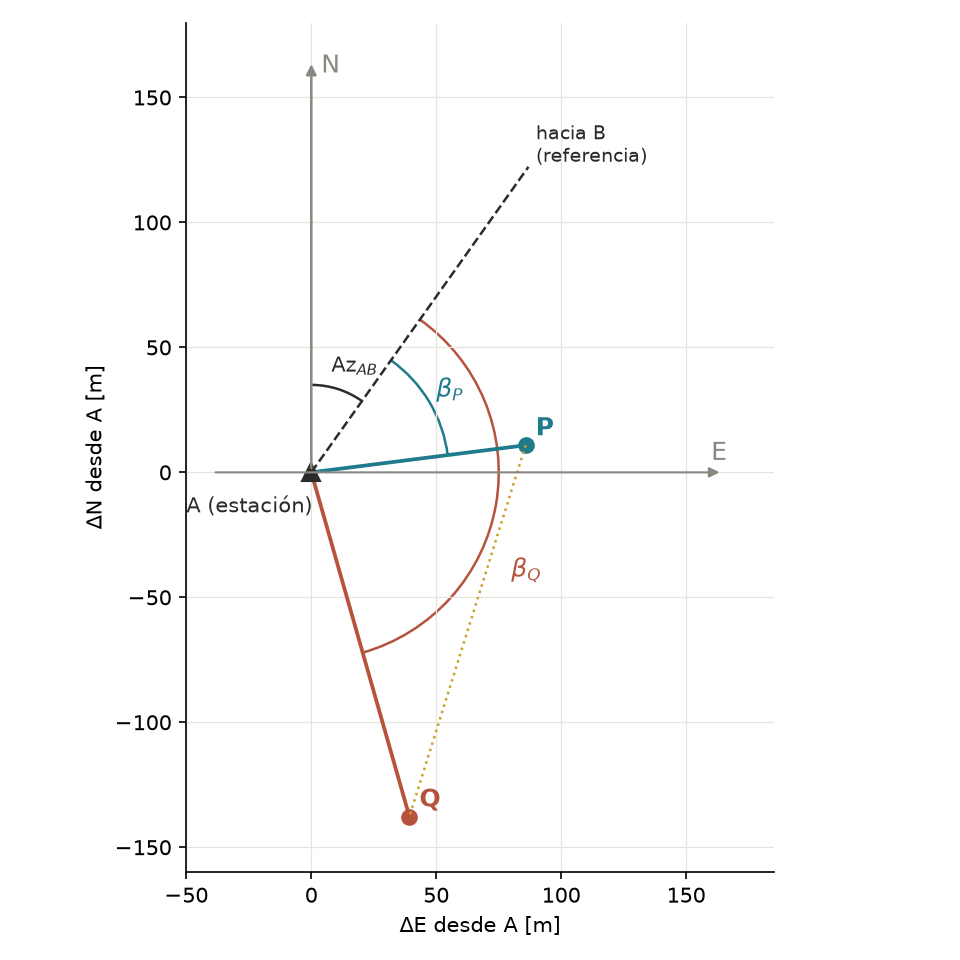
\includegraphics[width=.62\linewidth]{figuras/rotaciones/acimut_radiado.png}
\caption{Radiado desde la estación \(A\), en metros relativos a \(A\). La visual a la
referencia \(B\) tiene acimut \(\mathrm{Az}_{AB}\approx35^\circ\,24'\); los ángulos
\(\beta_P\) y \(\beta_Q\) se cuentan desde esa visual en sentido horario y llevan a \(P\) y
\(Q\). El segmento punteado \(PQ\) se usa en la verificación. Generada con
\texttt{apunte/scripts/cap01\_acimut\_estacion\_total.py}.}
\label{fig:acimut-radiado}
\end{figure}

\paragraph{Verificación: la rotación conserva distancias.} La distancia entre los dos puntos
radiados puede calcularse de tres maneras independientes.
\begin{itemize}
  \item Desde las coordenadas finales: \(\overline{PQ}=\sqrt{(E_Q-E_P)^2+(N_Q-N_P)^2}=155{,}699\) m.
  \item En el sistema propio del instrumento, con el eje \(y'\) hacia \(B\) y el \(x'\)
  perpendicular hacia la derecha: allí \(P'=R(-\beta_P)(0,d_P)=(63{,}624;\ 58{,}531)\) y
  \(Q'=R(-\beta_Q)(0,d_Q)=(111{,}780;\ -89{,}533)\), y \(\overline{P'Q'}=155{,}699\) m. Las
  coordenadas finales son \(A+R(-\mathrm{Az}_{AB})\,P'\) y \(A+R(-\mathrm{Az}_{AB})\,Q'\): un
  movimiento rígido, que por la proposición~\ref{prop:propiedades-R} no cambia la distancia.
  \item Solo con las medidas, por la ley del coseno en el triángulo \(APQ\), cuyo ángulo en
  \(A\) es \(\gamma=\beta_Q-\beta_P=81^\circ\,18'\,23{,}0''\):
  \(\overline{PQ}=\sqrt{d_P^2+d_Q^2-2\,d_Pd_Q\cos\gamma}=155{,}699\) m.
\end{itemize}
Los tres valores coinciden (la diferencia es menor que \(10^{-9}\) m), y también se recuperan
\(\overline{AP}=86{,}452\) m y \(\overline{AQ}=143{,}217\) m desde las coordenadas. La ley del
coseno es el producto interno de la sección~\ref{sec:interno} escrito con normas y ángulo; que
dé lo mismo es la conservación del producto interno por \(R\).

\paragraph{El cuadrante importa.} Para el acimut de \(P\) hacia \(Q\) los incrementos son
\(\Delta E=-46{,}515\) m y \(\Delta N=-148{,}588\) m. El cociente \(\Delta E/\Delta N\) es
positivo y \(\arctan(\Delta E/\Delta N)=17{,}382484^\circ\), que es la dirección opuesta: con
los dos incrementos negativos el punto \(Q\) está al sur y al oeste de \(P\), en el tercer
cuadrante. La función de dos argumentos da
\[
\mathrm{Az}_{PQ}=\operatorname{atan2}(-46{,}515;\ -148{,}588)=197{,}382484^\circ=197^\circ\,22'\,56{,}9'',
\]
y el acimut inverso es \(\mathrm{Az}_{QP}=17^\circ\,22'\,56{,}9''\). El valor ingenuo coincidía
con \(\mathrm{Az}_{QP}\): el error es exactamente media vuelta.

\unidadInteractiva{01a_punto_quieto}{Rotaciones I: el punto no se movió}{Explorá: girá los ejes un ángulo como el de orientación \(\mathrm{Az}_{AB}\) y comprobá que el punto queda quieto aunque cambien sus coordenadas, como pasa al llevar \(P'\) del sistema del instrumento al de la faja.}

\unidadInteractiva{02_producto_interno}{Producto interno: proyección, longitud, ángulo}{Verificá: con dos vectores de longitudes \(d_P\) y \(d_Q\) que formen el ángulo \(\gamma\), comprobá que la distancia entre sus extremos es la que da la ley del coseno.}

\section{En profundidad}

El apéndice~\ref{ap:infinitesimales} desarrolla las rotaciones infinitesimales y su relación
con la exponencial; el apéndice~\ref{ap:rot3d} construye las matrices de rotación 3D y la
fórmula de Rodrigues para un eje arbitrario.

\subsection{Rotaciones pequeñas}

\begin{definicion}[Generadores infinitesimales]
Los \emph{generadores} de las rotaciones elementales son las derivadas en \(\theta=0\):
\[
A_x=\left.\frac{dR_x}{d\theta}\right|_{0}=
\begin{pmatrix}0&0&0\\0&0&-1\\0&1&0\end{pmatrix},\quad
A_y=\left.\frac{dR_y}{d\theta}\right|_{0}=
\begin{pmatrix}0&0&1\\0&0&0\\-1&0&0\end{pmatrix},\quad
A_z=\left.\frac{dR_z}{d\theta}\right|_{0}=
\begin{pmatrix}0&-1&0\\1&0&0\\0&0&0\end{pmatrix}.
\]
\end{definicion}

\begin{proposicion}\label{prop:rot-pequenas}
Para un ángulo pequeño \(\varepsilon\),
\(R_x(\varepsilon)=I+\varepsilon A_x+O(\varepsilon^2)\), y lo mismo para \(y\) y \(z\).
Además, los dos órdenes de composición coinciden a primer orden y difieren a segundo orden en
\[
(I+\varepsilon A_x)(I+\varepsilon A_y)-(I+\varepsilon A_y)(I+\varepsilon A_x)
=\varepsilon^2(A_xA_y-A_yA_x)=\varepsilon^2A_z.
\]
\end{proposicion}

\begin{demostracion}
La primera afirmación es el desarrollo de Taylor de \(\cos\varepsilon=1+O(\varepsilon^2)\) y
\(\sin\varepsilon=\varepsilon+O(\varepsilon^3)\) en cada entrada (detalle en el
apéndice~\ref{ap:infinitesimales}). Al desarrollar los productos,
\((I+\varepsilon A_x)(I+\varepsilon A_y)=I+\varepsilon(A_x+A_y)+\varepsilon^2A_xA_y\), y el
orden inverso cambia solo el término \(\varepsilon^2A_yA_x\). Multiplicando las matrices,
\(A_xA_y\) tiene un único \(1\) en la posición \((2,1)\) y \(A_yA_x\) un único \(1\) en la
posición \((1,2)\); su diferencia es \(A_z\).
\end{demostracion}

\begin{ejemplo}[Cuánto no conmutan dos giros de \(0{,}01\) rad]
Con \(\varepsilon=0{,}01\), el cálculo exacto da
\(R_x(\varepsilon)R_y(\varepsilon)-R_y(\varepsilon)R_x(\varepsilon)\approx\varepsilon^2A_z\),
cuyas entradas no nulas son \(\mp0{,}0001\): cien veces menores que el giro mismo. Por eso las
rotaciones muy pequeñas parecen conmutar, aunque no conmutan exactamente; y la diferencia es,
ella misma, un giro pequeño alrededor del tercer eje.
\end{ejemplo}

\subsection{Eje de rotación, autovectores y exponencial}\label{sec:eje-exp}

\subsubsection{El eje como dirección fija}

\begin{definicion}[Rotación propia y eje]
Una matriz \(R\) de \(3\times3\) es una \emph{rotación propia} si \(R^TR=I\) y \(\det R=1\).
Un \emph{eje} de \(R\) es una dirección \(v\neq0\) con \(Rv=v\); en el lenguaje del
capítulo~\ref{cap:autovectores}, un autovector de autovalor \(1\).
\end{definicion}

\begin{teorema}[Euler]\label{teo:euler-eje}
Toda rotación propia de \(\R^3\) tiene un eje.
\end{teorema}

\begin{demostracion}
Hay que ver que \((R-I)v=0\) tiene solución no nula, es decir, que \(\det(R-I)=0\). Usando
\(R^TR=I\) y \(\det R=\det R^T=1\):
\[
\det(R-I)=\det\bigl(R^T(R-I)\bigr)=\det(I-R^T)=\det\bigl((I-R)^T\bigr)=\det(I-R)
=(-1)^3\det(R-I).
\]
Un número igual a su opuesto es cero.
\end{demostracion}

Para hallar el ángulo alcanza la traza: en una base ortonormal cuyo tercer vector es el eje,
\(R\) tiene un bloque \(R(\theta)\) de \(2\times2\) y un \(1\) en la diagonal, de modo que
\(\operatorname{tr}R=1+2\cos\theta\) (la traza no depende de la base;
sección~\ref{sec:cambio-base}).

\begin{ejemplo}[Eje y ángulo de una permutación de ejes]\label{ej:permutacion}
La matriz
\[
P=\begin{pmatrix}0&0&1\\1&0&0\\0&1&0\end{pmatrix}
\]
tiene columnas \(Pe_x=e_y\), \(Pe_y=e_z\), \(Pe_z=e_x\): permuta cíclicamente los ejes. Es
ortogonal con \(\det P=1\). El sistema \((P-I)v=0\) da \(v_3=v_1\), \(v_1=v_2\), \(v_2=v_3\):
el eje es \((1,1,1)\). La traza es \(0=1+2\cos\theta\), de modo que \(\cos\theta=-1/2\) y
\(\theta=120^\circ\).
\end{ejemplo}

\subsubsection{Exponencial de matrices}

\begin{definicion}[Exponencial de una matriz]
La exponencial de una matriz cuadrada \(A\) es la serie
\[
  e^A=I+A+\frac{A^2}{2!}+\frac{A^3}{3!}+\cdots,
\]
que converge para toda \(A\) (la norma del término \(k\)-ésimo está acotada por
\(\|A\|^k/k!\)). Un \emph{logaritmo} de \(R\) es una matriz \(A\) con \(e^A=R\).
\end{definicion}

Si \(R=e^A\), la familia \(e^{\tau A}\), \(0\le\tau\le1\), describe una trayectoria continua
desde la identidad hasta \(R\), y \(e^{A/n}\) es un paso pequeño que, aplicado \(n\) veces,
produce \(e^A\).

\begin{ejemplo}[La rotación plana como exponencial]
Sea \(J=\left(\begin{smallmatrix}0&-1\\1&0\end{smallmatrix}\right)\). Como \(J^2=-I\), las potencias pares de
\(\tau J\) son \(\pm\tau^{2m}I\) y las impares \(\pm\tau^{2m+1}J\); agrupando,
\[
e^{\tau J}=\Bigl(1-\frac{\tau^2}{2!}+\cdots\Bigr)I+\Bigl(\tau-\frac{\tau^3}{3!}+\cdots\Bigr)J
=\cos\tau\,I+\sin\tau\,J=R(\tau).
\]
Para \(\tau=\pi/6\) la serie sumada numéricamente da las entradas \(0{,}866\) y \(0{,}500\) de
\(R(30^\circ)\). El generador \(J\) es el análogo plano de \(A_z\).
\end{ejemplo}

\begin{proposicion}[Generador antisimétrico]\label{prop:generador}
Sea \(R\) la rotación de ángulo \(\theta\in[0,\pi)\) alrededor del eje unitario \(u\). Entonces
\(R=e^{A}\) con
\[
A=
\begin{pmatrix}
0&-\omega_z&\omega_y\\
\omega_z&0&-\omega_x\\
-\omega_y&\omega_x&0
\end{pmatrix},
\qquad \omega=(\omega_x,\omega_y,\omega_z)=\theta\,u,
\]
y es el único logaritmo antisimétrico con \(|\omega|<\pi\) (el \emph{logaritmo principal}).
El vector \(\omega\) indica el eje y su norma es el ángulo.
\end{proposicion}

La demostración combina la fórmula de Rodrigues del apéndice~\ref{ap:rot3d} con la relación
entre generadores y exponencial del apéndice~\ref{ap:infinitesimales}. Numéricamente, el
logaritmo se calcula con \texttt{scipy.linalg.logm}.

\begin{ejemplo}[Generador de la permutación \(P\)]
Para la matriz \(P\) del ejemplo~\ref{ej:permutacion}, \(\theta=2\pi/3\approx2{,}094\) y
\(u=(1,1,1)/\sqrt3\), de modo que
\(\omega=\tfrac{2\pi}{3\sqrt3}(1,1,1)\approx(1{,}209;\,1{,}209;\,1{,}209)\) y
\(|\omega|\approx2{,}094\) rad \(=120^\circ\).
\end{ejemplo}

\subsection{Experimento: muchos giros pequeños alrededor de los tres ejes}

Componemos muchas veces un mismo paso formado por tres giros pequeños e iguales,
\[
Q_\varepsilon
=R_z(\varepsilon)R_y(\varepsilon)R_x(\varepsilon),
\qquad \varepsilon=0{,}01,
\]
con \texttt{MMULT} en una planilla o con \texttt{numpy}. Por la
proposición~\ref{prop:rot-pequenas}, a primer orden
\(Q_\varepsilon\approx I+\varepsilon(A_x+A_y+A_z)\). La matriz \(A_x+A_y+A_z\) es la de la
proposición~\ref{prop:generador} con \(\omega=(1,1,1)\), cuya norma es \(\sqrt3\): cada paso
es, aproximadamente, un giro de \(\varepsilon\sqrt3\) alrededor de \((1,1,1)\). Después de
\(n\) pasos el ángulo acumulado es
\[
  \Theta\approx n\varepsilon\sqrt3.
\]
Para llegar a la permutación \(P\) del ejemplo~\ref{ej:permutacion} hace falta
\(\Theta=2\pi/3\), es decir \(n\approx(2\pi/3)/(0{,}01\sqrt3)\approx120{,}9\); el entero más
cercano es \(n=121\):
\[
  \Theta\approx121\cdot0{,}01\cdot\sqrt3
  \approx2{,}096\ \text{rad}
  \approx120{,}079^\circ.
\]
El producto exacto \(Q_\varepsilon^{121}\), calculado numéricamente, tiene eje
\(\approx(0{,}575;\,0{,}581;\,0{,}575)\), muy cerca de \((1,1,1)/\sqrt3\),
de componentes \(\approx0{,}577\), y ángulo \(\approx119{,}879^\circ\); sus entradas difieren de las de \(P\) en
menos de \(0{,}008\). La pequeña discrepancia es el término de segundo orden de la
proposición~\ref{prop:rot-pequenas}, acumulado a lo largo de los 121 pasos.

\subsection{Producto interno: incidencia}\label{sec:interno}

\unidadInteractiva{02_producto_interno}{Producto interno: proyección, longitud, ángulo}{Verificá: variá el ángulo \(\theta\) entre \(u\) y \(v\) y comprobá que el producto interno se anula cuando son perpendiculares.}

El producto interno sirve para proyectar y para decidir si dos vectores son ortogonales
(\(u\cdot v=0\)). En coordenadas homogéneas aparece un tercer uso.
Un punto se representa por una terna \(p=(x,y,w)^T\) y una recta \(ax+by+c=0\) por otra
terna \(\ell=(a,b,c)^T\). Son objetos distintos (se los suele dibujar con símbolos
distintos), pero ambos son vectores de \(\R^3\), y
\[
  \boxed{\ \ell\cdot p=ax+by+cw=0\quad\Longleftrightarrow\quad p\ \text{está en}\ \ell\ }.
\]
La ecuación cartesiana de la recta dice \enquote{el producto interno con la normal es
cero}. Ni \(\ell\) ni \(p\) cambian de significado si se los multiplica por un número, y la
condición tampoco.

\section{Ejercicios con solución}

\begin{ejercicio}
Calculá la imagen de \(p=(5,2)\) por la rotación de \(60^\circ\) alrededor de \(c=(2,-1)\) y
verificá que \(|p'-c|=|p-c|\).
\solucion{\(p-c=(3,3)\), \(R(60^\circ)(3,3)\approx(-1{,}098;\,4{,}098)\),
\(p'\approx(0{,}902;\,3{,}098)\); ambas distancias valen \(3\sqrt2\approx4{,}243\).}
\end{ejercicio}

\begin{ejercicio}
La matriz homogénea
\[
H=\begin{pmatrix}0&-1&4\\1&0&2\\0&0&1\end{pmatrix}
\]
representa una rotación. Hallá su
ángulo y su centro.
\solucion{La parte lineal es \(R(90^\circ)\). El centro resuelve
\((I-R)c=(4,2)\); con \(c=(x,y)\): \(x+y=4\), \(-x+y=2\), de donde \(c=(1,3)\); en efecto
\(H(1,3,1)^T=(1,3,1)^T\).}
\end{ejercicio}

\begin{ejercicio}
Un punto está a \(100\) m de una estación, en \(p=(100,0)\). Compará su rotación exacta en
\(\varepsilon=0{,}02\) rad con la aproximación \((I+\varepsilon J)p\),
\(J=\left(\begin{smallmatrix}0&-1\\1&0\end{smallmatrix}\right)\).
\solucion{Exacta \(\approx(99{,}980;\,2{,}000)\), aproximada \((100;\,2)\); el error es
\(\approx0{,}020\) m \(\approx\varepsilon^2\cdot100/2\), de segundo orden.}
\end{ejercicio}

\begin{ejercicio}
Calculá \(R_z(90^\circ)R_x(90^\circ)e_y\) y \(R_x(90^\circ)R_z(90^\circ)e_y\). ¿Conmutan?
\solucion{El primero da \(e_z\) (\(R_x\) lleva \(e_y\) a \(e_z\), que \(R_z\) deja fijo); el
segundo da \(-e_x\) (\(R_z\) lleva \(e_y\) a \(-e_x\), que \(R_x\) deja fijo). No conmutan.}
\end{ejercicio}

\begin{ejercicio}
Convertí el acimut \(\mathrm{Az}=230^\circ\) en ángulo matemático \(\theta\), y el ángulo
\(\theta=30^\circ\) en acimut.
\solucion{\(\theta=90^\circ-230^\circ=-140^\circ\equiv220^\circ\);
\(\mathrm{Az}=90^\circ-30^\circ=60^\circ\).}
\end{ejercicio}
